\chapter{Konzeption}
\label{chap:konzept}
    In diesem Kapitel wird das erarbeitete Konzept dieser Arbeit dargelegt. Basierend auf den 
    Anforderungen, die aus den Anwendungsfällen, den Experteninterviews und der Zielgruppenanalyse 
    erhoben wurden, werden die daraus generierten Überlegungen und Entscheidungen transparent 
    dargestellt. Durch die bereits erfolgten Schritte der Anforderungsanalyse (siehe Kapitel \ref{chap:anforderungsanalyse})
    sind erste Schritte der Konzeption abgeschlossen. 
    \\
    Zu Anfang des Kapitels wird das allgemeine Ziel eines Konzeptes, sowie das konkrete Ziel dieser Arbeit 
    erläutert. Anschließend 
    wird auf das Anwendungsumfeld des Systems, bzw. des Frameworks, (\ref{sec:anwendungsumfeld}) eingegangen, darunter 
    welche zusätzlichen Komponenten notwendig sind, damit das Framework in einer dafür vorgesehenen Umgebung sinnvoll 
    eingesetzt werden kann.
    % die abzudeckenden Funktionalitäten (\ref{sec:konzeptfunktionalitaet}), die 
    %aus den Anforderungen ermittelt wurden, eingegangen. 
    Darauf folgend wird anhand den 
    zugrundeliegenden Informationen und Anforderungen das Architekturkonzept (\ref{sec:architekturkonzept}) erläutert. %, sowie das 
    %Softwarekonzept (\ref{subsec:softwarekonzept}) erläutert. 
    Dabei wird auf verschiedene kontextabhängige Aspekte, sowie Sichtweisen der Anwender und des Frameworks eingegangen.
    Die Darstellung des Konzeptes stützt sich mit Diagrammen und Veranschaulichungen.
    %Des Weiteren werden die Hintergründe der 

\section{Ziel der Konzeption}
\label{sec:konzeptziele}
    Das Ziel einer Konzeption ist die Veranschaulichung von abstrakten Ideen, geistiger Entwürfe und Leitideen. 
    Hierbei werden aus den zugrundeliegenden Problemstellungen, Szenarien und Anforderungen Entwürfe und 
    Lösungsmöglichkeiten erarbeitet und identifiziert. Diese helfen bei der Aufstellung von notwendigen Schritten 
    und dienen als Grundlage zur Untermauerung und Darlegung von Entscheidungen. Somit wird Dritten der Kontext, die 
    Domäne und das zu lösende Problem, bzw. die Lösung dargestellt. 
    \\
    \linebreak
    Im Rahmen dieser Arbeit ist das Ziel des Konzeptes die Veranschaulichung der Entscheidungsfindung zur Lösung des vorliegenden 
    Sachverhaltes. Das Konzept 
    erarbeitet eine Lösung zur Implementierung einer Anwendung, die es ermöglicht, Automatisierungen, Regeln und Prozesse innerhalb eines 
    Firmenbüros zu koordinieren. Der Fokus liegt dabei verstärkt auf der einfachen Nutzung des Frameworks für den Anwender und 
    die uneingeschränkte Ausprägungsvielfalt von Regelprozessen. Dadurch kann der Anwender die vorgegebene Struktur nutzen, um individuelle 
    Sachverhalte zu realisieren, die in seinem Umfeld abzudecken sind.
    \\
    Hierfür wird der allgemeine Aufbau der Architektur skizziert und demonstriert, wie eine solche Lösung aussehen kann. 
    Unter Berücksichtigung der Forschungsfrage (siehe Abschnitt \ref{sec:forschungsfragen}) wird eine Möglichkeit offengelegt, mit der 
    ein Softwareentwickler neue Regeln entwickeln und dem System hinzufügen kann, ohne ein weiteres zu erlernendes Framework zu verwenden. 
    Dabei sollen die notwendigen Schritte und Interaktionen formalisiert und für den Entwickler vereinfacht werden. Mit der 
    Definition der Zielsetzung der Arbeit (siehe Abschnitt\ref{sec:zielsetzung}) wird die Abgrenzung deutlich. 
    \\
    \linebreak
    In folgender Darlegung %des Konzeptes 
    wird nochmals konkreter auf den Kontext als auch auf die Intension der Arbeit eingegangen. 
    % Das Ziel des Konzeptes ist es, dem Entwickler den Aufwand zur Erweiterung des Systems zu minimieren durch weitere 
    % Regeln und Abdeckung von Anwendungsfällen (Use Cases) und eine Struktur vorgeben. (ToDo's, Flexibilität in der 
    % Umsetzung (nicht wie Home Assistant und openHAB eher eingeschränkt)) 

%\section{Abzudeckende Funktionalitäten}
%\label{sec:konzeptfunktionalitaet}
    % Was soll der Entwickler machen können? 
    % Welche Grundlagen braucht er, um eine Regel implementieren zu können?
    % Welche Funktionen müssen gegeben sein, um die Struktur vorzugeben? 
    % Reicht ein Hinweis weöche Stellen angepackt werden müssen, um eine Regel hinzuzufügen? 
    
    %%%%%%%%%%%%%%%%%%%%%%%%%%%%%%%%%%%%%%%%%%%%%%%%%%%%%%%%%%%%%

    % ZIEL DES KONZEPTES: Ein Framework für Entwickler bereitzustellen, welches die Mächtigkeit für den Entwickler offen lässt, nicht einschränkt 
    % und dennoch Konfiguration und Ausführung umsetzt. Der Entwickler muss lediglich den Zustandsraum, die MQTT-Topics und die Regeln definieren.
    % Der Entwickler bekommt ein Framework in die Hand, welches die Umsetzung von Prozessen in einem smarten Büro ermöglicht. Das Framework kümmert sich um die 
    % Organisation und die Ausführung der Regeln. Die Richtigkeit der Regeln und des Zustandsraumes muss der Entwickler sicherstellen. 
    % Die Kommunikation über MQTT ist nur eine Möglichkeit. Des Setup wird wegabstrahiert 

    %%%%%%%%%%%%%%%%%%%%%%%%%%%%%%%%%%%%%%%%%%%%%%%%%%%%%%%%%%%%%

\section{Anwendungsumfeld}
\label{sec:anwendungsumfeld}
    Grundsätzlich ist der Einsatzort des Frameworks variabel, da die eigentliche Implementierung und Nutzung der Regeln und Prozesse stark 
    abhängig von den Anwendern ist. Dadurch kann sowohl im privaten \acl{SH} Umfeld als auch in Büroräumen ein System mittels dem 
    Framework erstellt werden. Basierend auf den vorangestellten Tätigkeiten, darunter die Anforderungsanalyse und die Eingrenzung auf den 
    Einsatz im Smart Office, liegt der Schwerpunkt der Arbeit auf dem Einsatz in einem smarten Büro. 
    \\
    \linebreak
    Stützend auf den vorab ermittelten Anwendungsfällen (siehe Abschnitt \ref{subsec:checkin} und \ref{subsec:evacuation}) sind unabhängige 
    Komponenten, darunter bspw. ein Service-Roboter und weitere einsatzfähige Geräte, sowie ein \acs{MQTT}-Broker notwendig. Ein \acs{MQTT}-Broker 
    wird im Zuge der Konzeption nicht von dem Framework bereitgestellt, lediglich die Anbindung als Client wird gegeben, und muss daher als eigenständige 
    Instanz bereitgestellt werden. Dadurch kann die Anforderung, die Kommunikation mittels \acs{MQTT}, ermöglicht werden. Eine mögliche infrastrukturelle 
    Architektur kann wie folgt aussehen: 
    \begin{figure}[hbt!]
        \centering
        
\includegraphics[width=14cm,height=11cm,keepaspectratio]{images/Systemarchitektur.png}
        \caption{Infrastruktur des Anwendungsumfeldes der Steuerzentrale}
        \label{fig:infrastructure}
    \end{figure}

\section{Konzept}
\label{sec:concept}
    Die Intension, die hinter der Ausarbeitung dieses Konzeptes steht, ist zum einen die einfache Handhabung der 
    formalisierten Interaktionen für Softwareentwickler %während
    unter der Verwendung des Frameworks und zum anderen die 
    offene Gestaltung von Regelprozessen, um so dem Anwender die Implementierung von Regeln und Aufgaben nicht 
    %einzugrenzen
    zu beschränken. Es soll lediglich ein Muster vorgegeben werden, damit Regeln einheitlich als solche von dem Framework 
    verarbeitet und genutzt werden können. 
    \\ 
    \linebreak
    In vergleichbaren Softwareprodukten, die im Rahmen dieser Arbeit erläutert 
    wurden (siehe Kapitel \ref{sec:homeassistant} und \ref{sec:openhab}), ist die Vielfalt der Regelausprägung auf 
    den Kontext des Systems eingeschränkt. Dies bedeutet, dass 
    Regeln und Prozesse nur mit Komponenten und Informationen innerhalb des Systems arbeiten können, bzw. benötigte 
    Informationen erst durch eine systemseitige Erweiterung durch Plugins verfügbar sind, auf die der Nutzer keinen direkten 
    Einfluss darauf nehmen kann. Diese Auswirkung ist unter anderem der 
    Tatsache geschuldet, dass mit den bestehenden Lösungen versucht wird, die Regeldefinition für Endnutzer so 
    einfach wie möglich zu gestalten. 
    \\
    \linebreak
    Um dennoch dem Anwender eine Struktur vorzugeben, mit der Regeln definiert und zur Laufzeit der Anwendung ausgeführt 
    werden können, soll mit diesem Konzept ein Framework erarbeitet werden, dass diese Herausforderung löst. Hierfür soll 
    dem Anwender die Komplexität der Regelverwaltung und deren Durchführung nicht vorgehalten werden. Dieser ist lediglich 
    in der Verantwortung, die für ihn notwendigen Regeln und Prozesse zu definieren und dem Framework bereitzustellen. 
    Dadurch soll der Person, die das Framework verwendet, die Möglichkeit geboten werden, das zur Verfügung gestellte System 
    mit individuellen Regeln, dafür vorgesehene Bedingungen, Komponenten und dessen Zustände zu implementieren. Beispielsweise 
    können bei Regeldefinitionen Informationen direkt von Datenpunkten über \acs{HTTP} Abfragen bezogen werden, bzw. Ressourcen 
    und Inhalte individuell nachgezogen werden.
    \\ 
    Das Konzept wird aus zweierlei Sichtweisen betrachtet, die in folgendem Abschnitt aufgegriffen werden und für die weitere 
    Konzepterläuterung notwendig sind.

    \subsection{Sichtweisen}
    \label{subsec:sichtweisen}
        Wie bereits aus dem Kontext hervorgeht, wird das Konzept auf zwei Sichtweisen aufgeteilt. Zum einen auf die 
        Anwendersicht, die der Softwareentwickler als entscheidende Kraft einnimmt, indem dieser das Aufsetzen und in 
        Betrieb nehmen des Systems, sowie das Definieren und Implementieren von Regeln übernimmt. Zum anderen die 
        Bereitstellungssicht, die das Framework als ausführende Kraft besetzt. Dieses sorgt für die Ausführung der vom 
        Anwender definierten Regeln. Ebenso stellt es Funktionen bereit, die das Empfangen von Events und das starten 
        von Regeln ermöglicht. Das Management zum Starten von Regeln und Prozessen wird in Gänze vom Framework übernommen. 
        Das Konzept widmet sich grundlegend dem initialen Aufbau des Frameworks. Zum besseren Verwalten und Starten von 
        Prozessen können weitere Konzepte und Managementroutinen ergänzt werden. Diese sind nicht Teil dieses Konzeptes und 
        werden im Ausblick zu möglichen Erweiterungsschritten nochmals aufgegriffen.
        \\
        \linebreak
        Zusammenfassend wird zwischen den beiden Sichtweisen differenziert, da diese Trennung ein elementarer Bestandteil des Konzeptes 
        aufzeigt. 
         % dafür, dass für das Setup benötigte Funktionen bereitstehen und vom Anwender definierte Regeln 
        %ausgeführt werden. 

    \subsection{Konzeptkomponenten}
    \label{subsec:conceptcomps}
        Für die Erläuterung des Konzeptes werden vorab die einzelnen Konzeptkomponenten erläutert, da diese die Anhaltspunkte 
        für den weiteren Verlauf darstellen. Das Framework baut auf folgenden Bausteinen auf:
        \begin{itemize} 
            \item Regel (Rule): Eine Regel ist ein Konstrukt, welches bei bestimmten Events die darin enthaltenen Aktionen ausführen soll. 
            Der grobe Aufbau einer Regel ist immer gleich. Diese beinhaltet einen Auslöser, eine Bedingung, einen Prozess und einen eindeutigen 
            Namen. Die Inhalte der Regel kann der Anwender ja nach bedarf beliebig ausprägen und ergänzen. 
            \item Komponente (Component): Eine Komponente bildet einen reellen Gegenstand ab, der bei Benutzung durch eine Regel für weitere Regeln 
            gesperrt und freigegeben werden kann. 
            \item Zustandsraum (State): Der Zustandsraum, das sog. Zustandsobjekt, bildet alle Zustände von Komponenten und weiteren Geräten ab. 
            \item Auslöser (Trigger): Der Auslöser ist ein von außen einwirkendes Objekt, das Zustandsänderungen hervorruft.
            \item Transformation (Transformer): Mit der Transformation werden eingehenden Events, die durch einen Auslöser hervorgerufen 
            werden und eine Zustandsänderung bewirken, auf das eigentliche Zustandsobjekt übertragen. 
        \end{itemize}
        In folgendem Abschnitt wird nochmals auf die Sichten eingegangen und anhand denen der Ablauf des Frameworks als auch die 
        Aufgaben des Anwenders erläutert. %Der Ablauf des Prozesses von Auslöser bis zur Ausführung der Regel wird anhand eines Programmablaufdiagramms gestützt.
        \\
        \linebreak
        Der Anwender hat das initiale Setup des Frameworks zur Aufgabe. Zuerst sollte der Zustandsraum erstellt werden. 
        Darin sollten alle notwendigen Zustände als Attribute und Objekte abgebildet sein. Nachdem das Zustandsobjekt 
        definiert wurde, geht es an die Definition und Implementierung der Regeln. Diese sind individuell, je nach 
        Anforderungen des Anwenders zu erstellen. Jedoch sind bestimmte Funktionen und Vorgaben bezüglich Bedingungsprüfung 
        und Prozessdurchlauf einzuhalten. Anforderungen dabei sind das Implementieren der beiden Funktionen, zum einen die 
        Bedingungen gegen Werte im Zustandsobjekt zu prüfen und zum anderen das Nutzen der Prozessfunktion, damit der Inhalt 
        der Regel durchlaufen wird.
        \\
        Nach Fertigstellung aller Regeln, müssen diese in einer Liste an das System übergeben werden. Anschließend sind die Kommunikationswege 
        zu aktivieren. 
        Da \acs{MQTT} zum aktuellen Zeitpunkt und zur Abdeckung der Anforderungen die einzige Kommunikationsschnittstelle abbildet, ist die 
        Konfiguration des \acs{MQTT} Clients einzustellen. Hierfür muss der Entwickler 
        dem Framework den Host des \acs{MQTT}-Brokers, sowie den Nutzername des Clients und dessen Passwort übergeben. Über das 
        Framework wird dann das Setup durchgeführt, sodass Topics, die über den Broker veröffentlicht werden, konsumiert werden können. 
        In Zuge dessen muss der Anwender alle Topics definieren und dem Framework übergeben. Dadurch wird gewährleistet, dass die 
        Steuerzentrale nur auf die Topics hört, die der Anwender bekannt gegeben hat. 
        \\
        Sind diese Schritte abgearbeitet, so sind die Pflichten des Anwenders erfüllt und die Steuerzentrale kann gestartet werden. 
        \\
        Hierfür wird der Durchlauf von dem Eingang einer \acs{MQTT} Nachricht bis zur Ausführung einer Regel aus Sicht des Frameworks erläutert.
        \\
        \linebreak
        textextextextextext.
        \begin{figure}[hbt!]
            \centering
            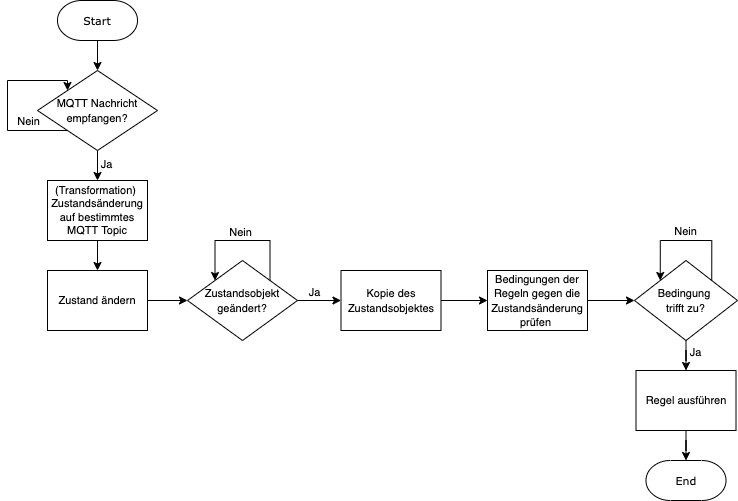
\includegraphics[width=14cm,height=11cm,keepaspectratio]{images/Programmablauf_Framework.png}
            \caption{Grober Programmablauf des Frameworks}
            \label{fig:programmablauf_framework}
        \end{figure}





\section{Architekturkonzept}
\label{sec:architekturkonzept}
    % Es wird alles abgebildet über einen Zustandsraum, der sich aus den Dingen (Gegenständen) und Zuständen der Anwendung ergibt.
    % Der Zustandsraum wird verändert, wenn eine Aktion durchgeführt wird, bzw. durch eine Trigger angestoßen. 
    % Bzw. speichert den aktuellen Zustand des Gegenstandes 
    % (lightBulb = true/false, personOnDoor = null/Mikka, booking = stringBooking, temiAktive = true/false, 
    % temiPosition = stringKoordinates)
    % Zustandsraum muss von dem Entwickler definiert werden. 
    % MQTT Broker über Home Assistant, bzw. losgelöster Broker
    % Anbindung von APIs auch Entwickler-Sache. Kann ich das vereinfachen, sodass die Integration einfacher wird?

    \subsection{Überlegungen, Anstöße und Herausforderungen}
    % Regeln über Thread abbilden? Ja, Nein? - Nein, wieso? Da Durch die MQTT Message mehrere Regeln ausgeführt 
    %werden können. -> Lediglich den Zustand der Komponenten locken.
    % KEIN THREAD (wird schon abgebildet durch die Services und die Auslöser durch MQTT), Falls eine Komponente 
    %  doppelt beansprucht wird, ist der Zustand der Komponenten zu locken und ein 
    % Thread.sleep einzurichten. Abfrage, ob der Wert, bzw. die Komponente wieder freigegeben wurde. 

    % Zustandsraum -> Abbildung aller notwendigen Komponenten 
    % Bei Bearbeitung einer Regeln die Komponenten Locken, sodass nur die einzelne Komponenten (deren Zustand) gelockt ist 
    % und nicht der ganze Zustandsraum, somit können mehrere Komponenten und Aktionen ausführen zu können. 

    %Was brauche ich für Funktionen und Werte in einer Regel?

    % Ein Zustandsraum (Objekt) für alles oder ein Globales, welches die die Komponenten enthält? - Begründung für die Auswahl.
    
    \subsection{Schnittstellen}
        % Kommunikation mit API's je nach Use Case und Gebrauch zur Datenabfrage
    
    \subsection{Datenbanken}
        % Datenbanken je nach Use Case und Gebrauch zur Datenabfrage

\subsection{Softwarekonzept}
\label{subsec:softwarekonzept}



